\section{Model Diagnostics \& Selection}
\subsection{Convergence Diagnostics (Gelman-Rubin, Trace Plots)}
We assessed the convergence of the three parallel MCMC chains using both quantitative metrics and visual inspection. The Gelman-Rubin statistic ($\hat{R}$) compares the variance within each chain to the variance between chains. It was preferred over single-chain diagnostics (Geweke), because of this inter-chain comparison \cite{silva2023notes}. Ideally, $\hat{R}$ should converge to 1.0, with values below 1.05 generally considered acceptable \cite{gelman2013}.
\begin{table}[h!]
	\centering
	\label{tab:convergence}
	\begin{tabular}{lcc}
		\hline
		\textbf{Parameter} & \textbf{Notation} & \textbf{$\hat{R}$ Estimate} \\
		\hline
		Intercept & $\beta_0$ & 1.02 \\
		Stabilized Glucose & $\beta_{SGLU}$ & 1.00 \\
		Age & $\beta_{AGE}$ & 1.01 \\
		Cholesterol & $\beta_{CHOL}$ & 1.01 \\
		Waist Circumference & $\beta_{WAIST}$ & 1.02 \\
		Systolic BP & $\beta_{SBP}$ & 1.01 \\
		Shape Parameter & $r$ & 1.00 \\
		\hline
	\end{tabular}
	\caption{Gelman-Rubin Convergence Diagnostics ($\hat{R}$) for the Gamma Regression Model.}
\end{table}

As presented in Table (1), all monitored parameters exhibited $\hat{R}$ point estimates between 1.00 and 1.02. These values confirm that the chains have fully converged to the stationary posterior distribution.

\begin{figure}[h!]
	\centering
	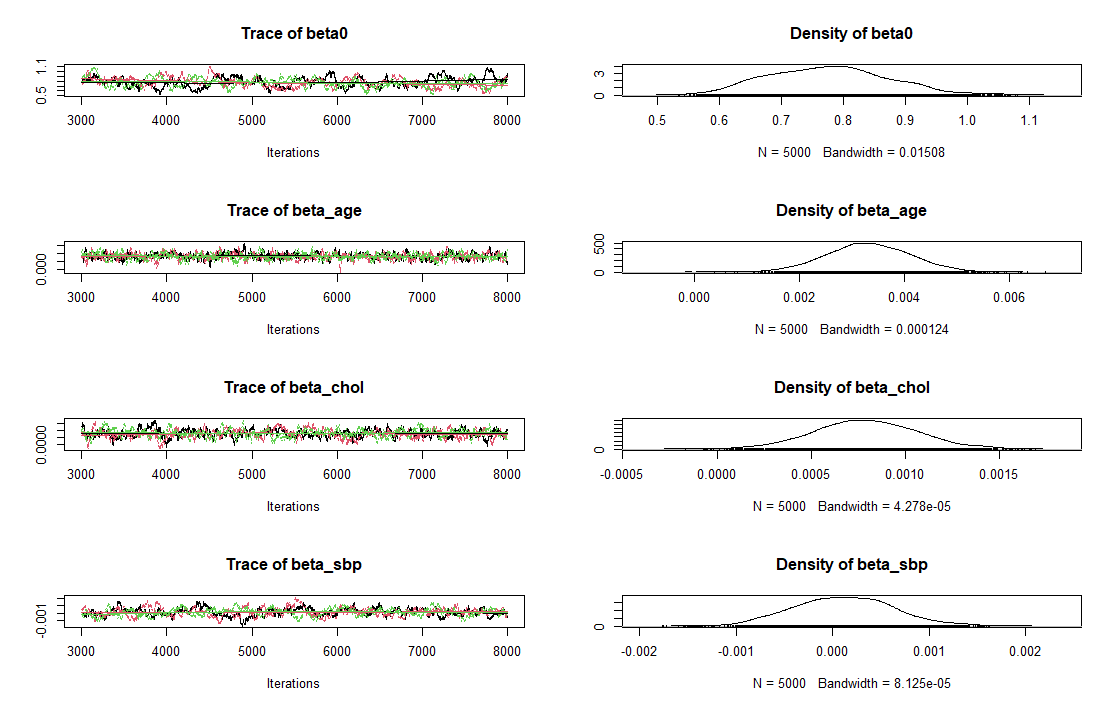
\includegraphics[width=1\linewidth]{Figures/Rplot1}
	\caption{Trace plots showing 5000 iterations after a total burn-in period of 3000 iterations (1000 adaptation + 2000 manual burn-in) (left column) and Posterior Density plots (right column) for some of the key parameters.}
	\label{fig:rplot1}
\end{figure}

\begin{figure}[h!]
	\centering
	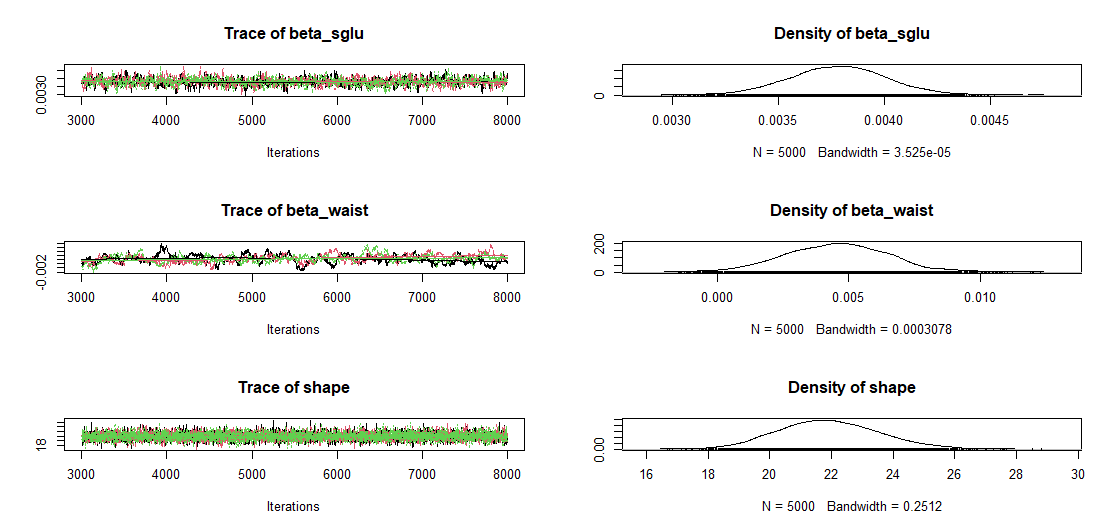
\includegraphics[width=1\textwidth]{Figures/Rplot2.png}
	\caption{Trace plots and Density plots for the SGLU ($\beta_{SGLU}$), Waist Circumference ($\beta_{WAIST}$), and shape ($r$).}
	\label{fig:rplot2}
\end{figure}
Complementing the numerical diagnostic, we visually examined the trace plots for some regression coefficients (Figure (\ref{fig:rplot1}) and (\ref{fig:rplot2})). The plots display the characteristic "fuzzy caterpillar" appearance, showing rapid fluctuations around a stable mean with no discernible trends or drifting. The three chains (represented by different colors) overlap significantly, indicating excellent mixing.

\subsection{Model Comparison (DIC)}
To select the most parsimonious model that balances goodness-of-fit with model complexity, we compared the Deviance Information Criterion (DIC) of the two candidate models. The DIC penalizes models with a higher number of effective parameters ($p_D$), favoring simpler models that fit the data well. The comparison results are as follows:

\begin{itemize}
	\item \textbf{Full Model (14 variables)}: DIC = 1154 ($p_D = 15.5$);
	\item \textbf{Reduced Model (5 variables)}: DIC = 1147 ($p_D = 7.2$).
\end{itemize}
The Reduced Model, i.e, our gamma model, presents a lower DIC value (1147 $<$ 1154). The lower penalty term ($p_D$) in the reduced model reflects its lower complexity compared to the full model. Since the reduced model achieves a better trade-off between deviance and complexity, it is selected as the final model for interpretation, adhering to the principle of parsimony. This confirms that the variables selected during the EDA are sufficient to explain the variability in GHB.

\section{Posterior Results and Clinical Interpretation}
Table (2) presents the posterior summaries for the parameters of the selected reduced model, based on 3 chains with 5000 iterations each (after a burn-in of 2000 iterations). The table includes the posterior mean, standard deviation (SD), and the 95\% Credible Interval (2.5\% and 97.5\% quantiles).
\begin{table}[h!]
	\centering
	\begin{tabular}{lcccc}
		\toprule
		\textbf{Parameter} & \textbf{Mean} $(\hat{\beta})$ & \textbf{SD} & \textbf{95\% Credible Interval} & \textbf{Conclusion} \\
		\midrule
		$\beta_0$       & 0.7764 & 0.0973 & $[0.6034, 0.9762]$   & Significant \\
		$\beta_{SGLU}$  & 0.0038 & 0.0002 & $[0.0033, 0.0042]$   & Significant \\
		$\beta_{AGE}$   & 0.0033 & 0.0008 & $[0.0018, 0.0049]$   & Significant \\
		$\beta_{CHOL}$  & 0.0008 & 0.0003 & $[0.0002, 0.0014]$   & Significant \\
		$\beta_{WAIST}$ & 0.0046 & 0.0020 & $[0.0007, 0.0086]$   & Significant \\
		$\beta_{SBP}$   & 0.0001 & 0.0005 & $[-0.0009, 0.0012]$  & Not Significant \\
		$r$ (shape)     & 21.920 & 1.6218 & $[18.891, 25.233]$   & -- \\
		\bottomrule
	\end{tabular}
	\caption{Posterior summaries of the Gamma Regression Model parameters (Reduced Model).}
\end{table}

The variables SGLU, Age, Cholesterol, and Waist Circumference all present 95\% Credible Intervals strictly greater than zero. This indicates a statistically significant positive association with GHB. The Systolic Blood Pressure (SBP) presents a posterior mean of $0.0001$, but its 95\% Credible Interval is $[-0.0009, 0.0012]$. Since this interval crosses zero, there is insufficient evidence in this model to conclude that SBP has a significant linear effect on GHB levels. Based on the posterior means, the estimated expected value of GHB is given by:
\begin{equation*}
	\eta_i = 0.776 + 0.0038 \cdot \text{SGLU}_i + 0.0033 \cdot \text{AGE}_i + 0.0008 \cdot \text{CHOL}_i + 0.0046 \cdot \text{WAIST}_i + 0.0001 \cdot \text{SBP}_i.
\end{equation*}

Although included in the mathematical formulation implies the posterior mean, the contribution of SBP is statistically negligible. Since the model uses a log link, the exponentiated coefficients ($\exp(\beta)$) provide a multiplicative interpretation. While a 0.4\% increase per unit of glucose might seem small, clinically relevant fluctuations are often larger. For example, an increase of 50 units in Stabilized Glucose (e.g., from 100 to 150 mg/dL) would result in an estimated increase in GHB of approximately 21\% ($1.0038^{50} \approx 1.208$), representing a substantial shift from healthy to diabetic levels. Similarly, each additional year of age is associated with a $0.3\%$ increase in GHB. The shape parameter $r$ was estimated at 21.92. Clinically, this value implies a relatively low Coefficient of Variation ($CV \approx 1/\sqrt{21.92} \approx 21\%$) \cite{gelman2013}, suggesting that GHB levels are regulated around the mean for the majority of the population. Contrary to an Exponential distribution ($r=1$) which would imply biological heterogeneity, this large shape parameter indicates that physiological homeostasis maintains GHB levels in a stable range, while the Gamma tail still has the right-skewness of diabetic outliers.